\section{Detailed Experiment Settings}
\label{sec:hyps}
We use a linearly decreasing learning rate initialized with 5e-4 on the research paper stream and 3e-4 on the tweet stream. On the research paper stream, we train the model for 8,000 steps in the first task, and 4,000 steps in the subsequent tasks. On the tweet stream, we train the model for 8,000 steps in all tasks. We hold out 128,000 sentences from each corpus to evaluate MLM performance. As the size of pretraining corpora is large, during training, each training example is visited only once. We use the masked language modeling perplexity over held-out validation sets of the pretraining corpora as the metrics for hyperparameter tuning. 
Common hyperparameters such as learning rate and batch sizes are tuned with Task-specific models with the first task. Hyperparameters that are specific to continual learning algorithms, such as the scale of the distillation loss, is tuned using the first two domains in the stream according to the MLM performance over validation sets. The weight of the distillation term $\alpha$ is set as 1.0 for logit distillation and 0.1 for other distillation algorithms. By default, we replay or perform distillation with a mini-batch of examples from the replay memory every 10 training steps in ER and Distillation-based CL approaches. We use the huggingface transformers library \url{https://github.com/huggingface/transformers} for implementation.
%\xiang{1-2 sentences on how hps of all the methods are determined; what metrics/loss we looked at.}
%In contrastive distillation approaches, we set $\alpha$=1 and $\tau$=0.05.

%Note that the label space of hashtag prediction can be different between years. In our experiments, for evaluation of temporal generalization, we use the label set of the earlier year, and collect examples from the held-out 1M tweets in the latest year that have at least one of the hashtags in the earlier year. We sub-sample 10,000 examples as the test set.



\section{Low-Resource Fine-Tuning}
\label{apdx:low_resource}


%xiang{\paragraph{\textit{Q5: Will continually pretrained model adapt faster to a new domain?}}
%--> pretraining data efficiency comparison between a continually pretrained model vs. roberta, when further pretrained to a new domain
%}
\begin{figure}[]
    \centering
    % \scalebox{0.9}{
    \subfloat[\scriptsize{Chemprot}]{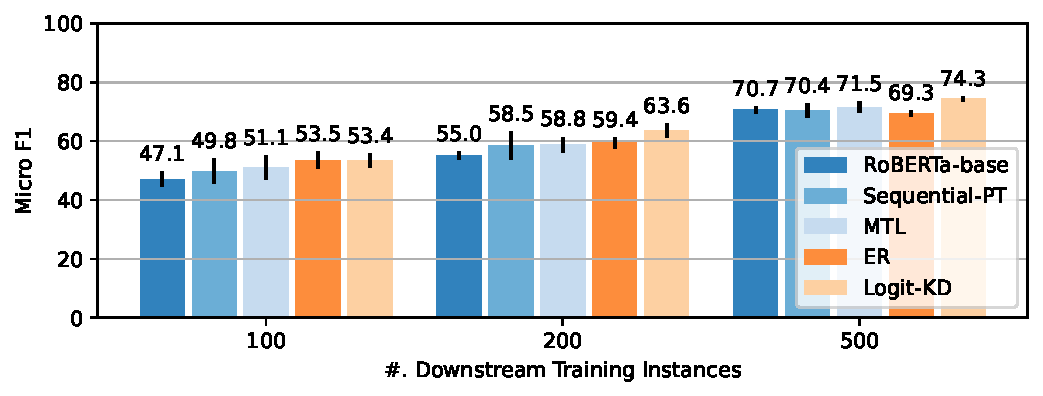
\includegraphics[width=0.94\linewidth]{acl2022/figs/academics_kshots/kshot_chemprot.pdf}}
    
    %\subfloat[\scriptsize{RCT-Sample}]{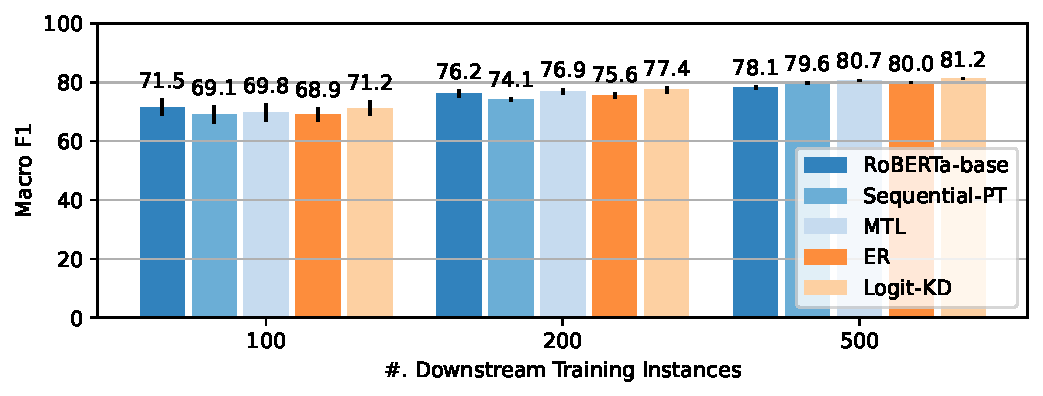
\includegraphics[width=0.94\linewidth]{acl2022/figs/academics_kshots/kshot_rct-sample.pdf}}
    
    %\vspace{-0.3cm}
    %\subfloat[\scriptsize{ACL-ARC}]{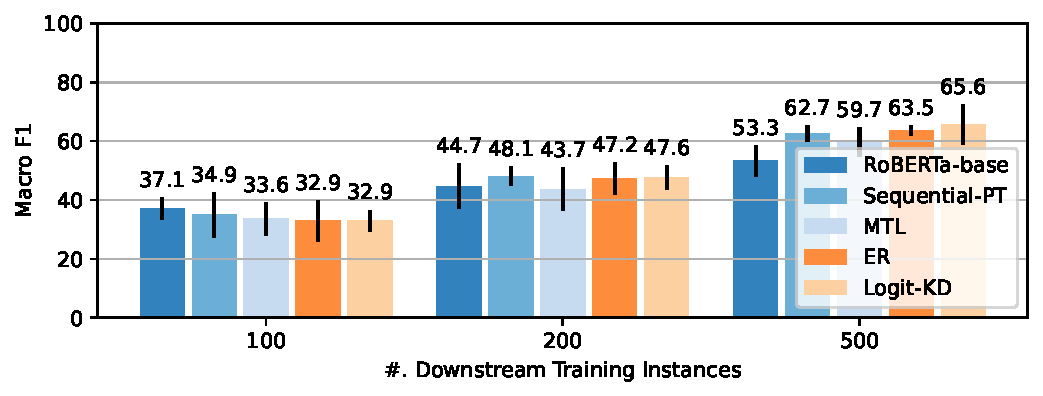
\includegraphics[width=0.94\linewidth]{acl2022/figs/academics_kshots/kshot_citation_intent.pdf}}
    % \vspace{-0.3cm}
    
    \subfloat[\scriptsize{SciERC}]{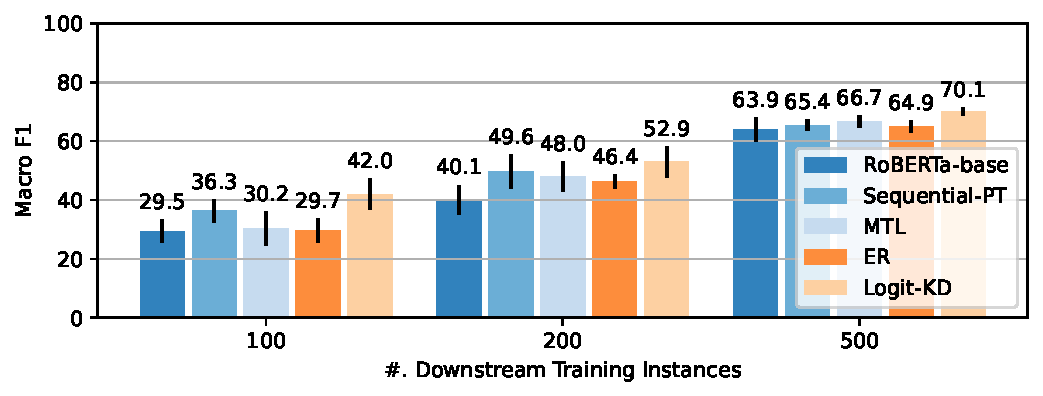
\includegraphics[width=0.94\linewidth]{acl2022/figs/academics_kshots/kshot_sciie.pdf}}
    % }
    \caption{\small Performance of downstream models with various number of training examples. The models are fine-tuned from the final pretrained model ($f_4$).}
    \label{fig:academics_kshot}
\end{figure}

Figure~\ref{fig:academics_kshot} summarizes the performance of fine-tuned models from the final model checkpoint ($t=4$) using different amount of downstream training examples. We see on Chemprot and SciERC, the benefit of Sequential Pretraining over RoBERTa-base is more significant in low-resource fine-tuning setups. 
%while on RCT-Sample and ACL-ARC, Sequential Pretraining improves over RoBERTa-base when there are sufficient amount of training examples. 
Whenever Seqential Pretraining outperforms RoBERTa-base, we notice Logit-KD could further improve over Sequential Pretraining.

\section{Full Results over the Tweet Stream}
\label{apdx:full_tweet_results}
\begin{table}[]
\centering
\scalebox{0.66}{
\begin{tabular}{@{}lcccc@{}}
\toprule
Task          & 2014                 & 2016                 & 2018                 & 2020                 \\ \midrule
\multicolumn{5}{c}{Hashtag Prediction}                                                      \\ \midrule
RoBERTa-base  & 56.65$_{\pm 0.6}$            & 45.50$_{\pm 2.1}$            & 48.08$_{\pm 1.0}$            & 56.42$_{\pm 0.2}$            \\
Sequential PT        & 59.00$_{\pm 0.1}$            & 54.28$_{\pm 0.3}$            & 56.79$_{\pm 0.5}$            & 59.85$_{\pm 0.4}$            \\
ER            & 59.00$_{\pm 0.1}$            & 54.90$_{\pm 0.2}$            & 56.93$_{\pm 0.1}$            & 59.56$_{\pm 1.7}$            \\
Adapter       &     58.76$_{\pm 0.7}$         &         52.55$_{\pm 1.5}$             &           54.34$_{\pm1.7}$           &          59.01$_{\pm 1.0 }$            \\
Logit-KD      &   60.93$_{\pm 0.5}$        &        55.96$_{\pm 0.2}$              &            58.21$_{\pm 0.5}$          &        60.52$_{\pm 0.2}$              \\
Rep-KD        &      60.47$_{\pm 0.1}$           &      51.77$_{\pm 2.6}$                &              55.79$_{\pm 1.4}$        &          59.80$_{\pm 0.2}$ \\
Contrast-KD   &       60.72$_{\pm 0.6}$         &      55.85$_{\pm 0.0}$              &         57.94$_{\pm 0.4}$         &     59.54$_{\pm 0.3}$                 \\
SEED-KD & 58.82$_{\pm 0.4}$ & 54.55$_{\pm 0.5}$ & 56.87$_{\pm 0.2}$ & 59.71$_{\pm 0.2}$ \\
SEED-Logit-KD &        61.28$_{\pm 0.2}$           &            55.59$_{\pm 0.5}$          &                57.75$_{\pm 0.4}$      &          60.74$_{\pm 0.6}$            \\
Task-Specific (2014) & 61.62$_{\pm 0.3}$            & 55.38$_{\pm 0.6}$            & 56.16$_{\pm 0.6}$            & 59.59$_{\pm 0.3}$            \\
Task-Specific (Latest) & 59.91$_{\pm 0.3}$            & 55.47$_{\pm 1.0}$            & 56.61$_{\pm 0.4}$            & 59.87$_{\pm 0.6}$            \\
MTL           & 60.51$_{\pm 0.3}$            & 55.16$_{\pm 1.6}$            & 57.89$_{\pm 0.4}$            & 59.95$_{\pm 0.3}$            \\ \midrule
               \multicolumn{5}{c}{Emoji Prediction}                                                      \\ \midrule
RoBERTa-base  & 28.73$_{\pm 0.2}$            & 26.86$_{\pm 0.2}$            & 25.71$_{\pm 0.1}$            & 24.42$_{\pm 0.2}$            \\
Sequential PT       & 32.69$_{\pm 0.2}$            & 30.55$_{\pm 0.3}$            & 29.30$_{\pm 0.1}$            & 27.69$_{\pm 0.1}$            \\
ER            & 32.88$_{\pm 0.2}$            & 30.52$_{\pm 0.2}$            & 29.50$_{\pm 0.1}$            & 27.75$_{\pm 0.1}$            \\
Adapter       &      32.15$_{\pm 0.2}$         &        29.85$_{\pm 0.0}$         &            28.72$_{\pm 0.0}$          &     26.80$_{\pm 0.3}$             \\
Logit-KD      & 33.08$_{\pm 0.3}$            & 30.88$_{\pm 0.1}$            & 29.77$_{\pm 0.1}$            & 27.80$_{\pm 0.1}$            \\
Rep-KD        &      32.71$_{\pm 0.2}$         &        30.51$_{\pm 0.2}$              &        29.45$_{\pm 0.1}$          &        27.27$_{\pm 0.2}$          \\
Contrast-KD   & 32.90$_{\pm 0.1}$            & 31.01$_{\pm 0.1}$            & 29.48$_{\pm 0.2}$            & 27.72$_{\pm 0.3}$            \\
SEED-KD & 32.91$_{\pm 0.1}$ & 30.84$_{\pm 0.3}$ & 30.12$_{\pm 0.1}$ & 27.66$_{\pm 0.1}$ \\
SEED-Logit-KD &      33.28$_{\pm 0.1}$          &      31.17$_{\pm 0.1}$                &           29.98$_{\pm 0.1}$       &       27.84$_{\pm 0.2}$               \\
Task-Specific (2014) & 33.37$_{\pm 0.2}$            & 30.54$_{\pm 0.3}$            & 28.94$_{\pm 0.0}$            & 26.98$_{\pm 0.2}$            \\
Task-Specific (Latest) & 32.31$_{\pm 0.0}$            & 29.83$_{\pm 0.5}$            & 29.06$_{\pm 0.2}$            & 27.19$_{\pm 0.1}$            \\
MTL           &  32.78$_{\pm 0.1}$  & 30.54$_{\pm 0.0}$ & 29.52$_{\pm 0.2}$ &  27.47$_{\pm 0.0}$ \\  \bottomrule
\end{tabular}
}
\caption{\small Full performance on Twitter Hashtag prediction and Emoji prediction, fine-tuned from the pre-trained model in the final time step.}
\label{tab:twitter_full}
\end{table}



% \begin{table}[]
% \centering
% \scalebox{0.72}{
% \begin{tabular}{@{}lcccc@{}}
% \toprule
%           \textbf{Tweet year}  & \textbf{2014}      & \textbf{2016}      & \textbf{2018}      & \textbf{2020}      \\ \midrule
% Roberta-base & 56.65$_{\pm 0.6}$ & 45.50$_{\pm 2.1}$ & 48.08$_{\pm 1.0}$ & 56.42$_{\pm 0.2}$ \\
% Naive CL     & 59.00$_{\pm 0.1}$ & 54.28$_{\pm 0.3}$ & 56.79$_{\pm 0.5}$ & \textbf{59.85}$_{\pm 0.4}$ \\
% ER           & 59.00$_{\pm 0.1}$ & 54.90$_{\pm 0.2}$ & 56.93$_{\pm 0.1}$ & 59.56$_{\pm 1.7}$ \\
% %Logit-KD &   58.53$_{\pm 0.3}$     &    54.14$_{\pm 0.2}$   &  55.24$_{\pm 0.6}$         &    57.80$_{\pm 0.8}$     \\ 
% Logit-KD$_{\text{first}}$ &   \textbf{59.31}$_{\pm 2.4}$     &    \textbf{55.12}$_{\pm 0.5}$   &  \textbf{56.99}$_{\pm 0.2}$         &    59.77$_{\pm 0.5}$     
% \\ 
% \midrule
% Task-Specific LM      &   59.91$_{\pm 0.3}$    & 55.47$_{\pm 1.0}$ & 56.61$_{\pm 0.4}$ & 59.87$_{\pm 0.6}$ \\ \bottomrule
% \end{tabular}
% }


% \end{table}
\begin{table}[]
\centering
\scalebox{0.66}{
\begin{tabular}{@{}lccc@{}}
\toprule
Task          & 2014 $\to$ 2020 & 2016 $\to$ 2020 & 2018 $\to$ 2020 \\ 
\midrule
\multicolumn{4}{c}{Crossyear Hashtag Prediction}                        \\
\midrule
RoBERTa-base  & 39.31$_{\pm 2.7}$     & 42.23$_{\pm 2.7}$     & 37.19$_{\pm 2.1}$     \\
Sequential PT       & 44.00$_{\pm 1.1}$     & 49.87$_{\pm 1.8}$     & 46.63$_{\pm 0.9}$     \\
ER            & 43.31$_{\pm 0.2}$     & 50.72$_{\pm 0.6}$     & 46.27$_{\pm 0.4}$     \\
Adapter       &    42.61$_{\pm 0.5}$           &        48.00$_{\pm 1.6}$       &   42.63$_{\pm 0.9}$            \\
Logit-KD      & 44.26$_{\pm 0.9}$     & 50.92$_{\pm 0.8}$     & 46.84$_{\pm 1.0}$     \\
Rep-KD        &     42.48$_{\pm 0.2}$      &        50.38$_{\pm 1.5}$       &       42.23$_{\pm 0.2}$        \\
Contrast-KD   &      45.22$_{\pm 0.1}$       &       52.14$_{\pm 1.1}$         &            47.47$_{\pm 0.8}$   \\
SEED-KD & 43.39$_{\pm 0.4}$  & 49.62$_{\pm 1.0}$ & 46.37$_{\pm 0.8}$ \\
SEED-Logit-KD &   45.35$_{\pm 0.6}$      &      51.56$_{\pm 0.7}$     &         47.74$_{\pm 0.3}$      \\
Task-Specific (2014) &      44.34$_{\pm 0.6}$         &         49.26$_{\pm 0.7}$      &        45.09$_{\pm 0.7}$       \\
Task-Specific (2020) &      43.44$_{\pm 0.5}$          &           49.41$_{\pm 1.1}$                &          44.34$_{\pm 0.4}$        \\
- \textit{4x steps}& 44.34$_{\pm 0.6}$     & 51.78$_{\pm 0.7}$     & 44.69$_{\pm 0.7}$     \\
MTL           & 44.04$_{\pm 0.3}$     & 50.37$_{\pm 0.3}$     & 44.31$_{\pm 0.0}$     \\ 
\midrule
\multicolumn{4}{c}{Crossyear Emoji Prediction}                          \\ \midrule
RoBERTa-base  & 12.02$_{\pm 0.4}$     & 13.24$_{\pm 0.2}$     & 18.67$_{\pm 0.1}$     \\
Sequential PT       & 14.20$_{\pm 0.2}$     & 16.08$_{\pm 1.4}$     & 21.06$_{\pm 0.9}$     \\
ER            & 14.36$_{\pm 0.4}$     & 16.82$_{\pm 0.3}$     & 21.57$_{\pm 0.1}$     \\
Adapter       &     13.53$_{\pm 0.2}$       &   15.68$_{\pm 0.3}$        &      20.64$_{\pm 0.1}$         \\
Logit-KD      & 14.20$_{\pm 0.3}$     & 16.28$_{\pm 1.1}$     & 21.29$_{\pm 1.0}$     \\
Rep-KD        &    13.89$_{\pm 0.1}$       &        16.03$_{\pm 0.3}$       &           20.86$_{\pm 0.2}$    \\
Contrast-KD   &     14.42$_{\pm 0.3}$       &       17.52$_{\pm 0.1}$        &      21.43$_{\pm 0.1}$         \\
SEED-KD & 14.36$_{\pm 0.1}$ & 16.97$_{\pm 0.4}$ & 21.88$_{\pm 0.3}$ \\
SEED-Logit-KD & 14.36$_{\pm 0.1}$    &     16.97$_{\pm 0.3}$      &         21.62$_{\pm 0.1}$      \\
Task-Specific (2014) &    13.39$_{\pm 0.2}$        &        15.14$_{\pm 0.2}$                   &       20.79$_{\pm 0.3}$              \\
Task-Specific (2020) & 13.00$_{\pm 0.2}$     & 14.48$_{\pm 0.3}$     & 19.30$_{\pm 0.2}$     \\
- \textit{4x steps}& 12.90$_{\pm 0.4}$     & 14.85$_{\pm 0.3}$     & 19.83$_{\pm 0.2}$     \\
MTL           &     14.07$_{\pm 0.2}$       &       16.64$_{\pm0.2}$    &       20.94$_{\pm 0.7}$   \\ 
\bottomrule
\end{tabular}
}
\caption{\small Temporal generalization performance on Twitter Hashtag prediction datasets fine-tuned from the final pre-trained model. \texttt{Year 1}$\to$\texttt{Year 2} indicates the hashtag prediction model is fine-tuned on data in year \texttt{Year 1}, and evaluated on test data in \texttt{Year 2}.}
\vspace{-0.3cm}
\label{tab:twitter_tg_full}
\end{table}

Tables~\ref{tab:twitter_full} and~\ref{tab:twitter_tg_full} summarize full results over the Tweet stream. Compared to the table~\ref{tab:twitter} in the main text, we add downstream performance over data from years 2014 and 2016 ($D_1$, $D_2$), and temporal generalization from year 2014 to 2020 ($D_1 \to D_4$). 

\section{Dataset Details}
\label{apdx:dataset_details}
The research paper stream consists of full text of 6.6M, 12.1M, 7.8M, and 7.5M research papers from the S2ORC~\cite{Lo2020S2ORCTS} dataset. We evaluate downstream fine-tuning performance on two in-domain datasets for each research area:
Chemprot relation exaction dataset~\cite{Vindahl2016ChemProt30AG} and RCT abstract sentence role labeling dataset ~\cite{Dernoncourt2017PubMed2R} for the bio-medical domain; 
ACL-ARC citation intent classification dataset~\cite{Jurgens2018MeasuringTE} and SciERC relation extraction dataset~\cite{Luan2018MultiTaskIO} for the computer science domain; 
relation extraction over Synthesis procedures~\cite{mysore2019materials} and named entity recognition over material science papers (MNER)~\cite{olivetti2020data} for material science domain; keyphrase classification and hyponym classification after filtering out physics papers for the physics domain~\cite{augenstein2017semeval}. We report micro-averaged F1 on Chemprot, RCT, MNER datasets following the evaluation metrics in the original work, and report macro-averaged F1 on all other datasets. We use the official data splits for all datasets except for RCT, where we employ a low-resource training setup following~\citet{Gururangan2020DontSP}. %\xiang{say a bit on the train/test splist for these datasets?}

The pretraining corpora for the tweet stream consist of 25M tweets in each year. 
For downstream tasks, we use a separate set of 1M tweets from each year to construct multi-label hashtag prediction~\cite{Gong2016HashtagRU} datasets and single-label emoji prediction datasets~\cite{Barbieri2018SemEval2T}. We replace user names to special tokens. For Hashtag prediction, the label space consists of tweets containing 200 most frequent hashtags in each year. We independently sample 500 tweets per label (hashtag) as training, validation and test sets, which results 10$k$ examples in each of the data splits. For emoji prediction, we construct 20-way single-label emoji prediction datasets for each year following~\citet{Barbieri2018SemEval2T} with the 1M held out tweets. We sample 5,000 tweets per emoji in each split, resulting in balanced datasets of the same size as the hashtag prediction datasets.
%\xiang{add a line to point to appendix for more details on the dataset construction and the full list of hashtags used in our exps.}

\section{Details of Continual Learning Algorithms}
\label{apdx:cl}
\subsection{Contrastive Distillation}
During continual pretraining, in addition to the language model pretraining objective, we add a unsupervised contrastive learning objective, namely the SimCSE~\cite{Gao2021SimCSESC} objective, so that the similarity in the sentence representation better reflects the semantic similarity in the sentence. 
We use the $l^2$-normalized representation of the start-of-sequence token at the final layer as the sentence representation, noted as $\bm{h}$. Then, we distill the intra-batch representational similarity from the previous model $f_{t-1}$ to the current model $f_t$. Given a mini-batch of $N$ examples $\bm{x}$, we compute the representational dot-product similarity matrix between normalized sentence representations $\bm{h}$ between each pair of examples with $f_{t-1}$ and $f_t$, noted as $\mathbf{B}^{t-1}$ and $\mathbf{B}^{t}$, where each element $\mathbf{B}_{ij}$ is, 
\begin{equation}
    \label{eq:normalize}
    \mathbf{B}_{ij} = \frac{\exp(\bm{h}_i \cdot \bm{h}_j / \tau)}{\sum_{k=1..N}\exp(\bm{h}_i \cdot \bm{h}_k / \tau)}
\end{equation}
where $\tau$ is a temperature hyperparameter. We specify a temperature $\tau_t=0.05$ for the teacher model $f_{t-1}$ and a temperature $\tau_s$ for the student model $f_t=0.01$. We compute the cross-entropy between $\mathbf{B}^{t-1}$ and $\mathbf{B}^{t}$ as the distillation loss,
\begin{equation}
    \label{eq:contrastive_distill}
    \ell_{\text{distill}} = - \frac{1}{N} \sum_{i=1}^{N} \sum_{j=1}^{N} \mathbf{B}_{ij}^{t-1}\log \mathbf{B}_{ij}^{t}
\end{equation}

\subsection{SEED Distillation}
SEED distillation proposed by~\cite{Fang2021SEEDSD} has a similar spirit as the contrastive distillation with differences in the examples used for computing similarity matrices computes. The algorithm distills representational similarity \textit{between the batch and a large set of other examples}, maintained in an example queue $Q$.
As the number of target examples $K$ can be much larger than the batch size, it allows distillation of richer information by regularizing similarities. During pretraining, the method maintains a fixed-size queue $Q$ to cache examples from the current domain $D_t$. Given a mini-batch of training examples $\bm{x}$, it computes cosine similarity between each pair of examples within the batch $\bm{x}$ and $Q$ with $f_{t-1}$ and $f_{t}$, resulting in two similarity matrices $\mathbf{B}^{t-1}$, $\mathbf{P}^y \in \mathbb{R}^{|B|\times |Q|}$. Similar to the contrastive distillation, the distillation loss is the cross-entropy between two similarity matrices $\mathbf{B}^{t-1}$ and $\mathbf{B}^{t}$ computed in the same way as Eq.~\ref{eq:contrastive_distill}. 


\section{Analysis and Controlled Experiments of Computational Costs}
\label{apdx:controlled_computation_costs}

Computational cost is a crucial matter for online continual learning systems. In this section, we analyze the computational costs of continual learning algorithms and perform controlled experiments of computational costs.

We quantify computational costs with the total number of \textit{forward ($C_f$) and backward ($C_b$)} computations ($C=C_f+C_b$) over the PTLMs, which is easy to control; in practice, we find the wall clock time of training was approximately linear to $C$. We summarize the number of forward and backward passes and the wall clock time of training in Table~\ref{tab:forward_backward_count}. In the visit of $b$ batches from the training stream, Sequential PT performs $b$ forward and backward passes respectively over the PTLM, resulting in $C=2b$. Experience replay further replays 1 batch of examples every $k$ steps over the training stream, which results in $C=(2+2/k)b$. In our main experiments, $r$ is set to 10 (Sec.~\ref{ssec:mem_replay_methods}). Logit-Distill and Rep-Distill require one additional forward pass over a frozen PTLM to compute the target of distillation, resulting in $C=(3+3/k)b$. Distillation algorithms that perform contrastive learning with SimCSE (\textit{i.e.} SEED-Distill and SEED-Logit-Distill) additionally require one forward and backward pass using the same batch of examples with different dropout masks. Therefore, for SEED-Logit-Distill, $C=(5+5/k)b$.

To control the number of forward and backward passes, we present approaches to compensate the lower computation costs compared to Distillation algorithms and one approach to shrink the computational cost of distillation algorithms: (1) for Sequential PT, we train the models for 1.2 times more steps so that $C=2.4b$, noted as Sequential PT$_{b^\prime=1.2b}$; (2) for ER, we increase the replay frequency $k$ to 5 from the default setup 10, so that $C=2.4b$. We also decrease the cost of Logit-KD and SEED-Logit-KD by reducing the frequency of distillation from every 1 batch to every $r^\prime=$10 steps, while still replaying and distilling knowledge over 1 batch of memory examples every 10 training steps. This results in $C_f=(1+2/k+1/k^\prime)b$ and $C_b=(1+1/k)b$, where $C=2.4b$ when both $r$ and $r^\prime$ are 10. The approach is referred to as Sparse Logit-KD. Finally, for SEED-Logit-KD, we remove the SimCSE loss from training and perform sparse distillation similar to Sparse-Logit-KD, which also results in $C=2.4b$.

The performance of the models is presented in Table~\ref{tab:controlled_results}. We notice that at the end of pretraining, increasing the number of training steps in Sequential PT by 1.2 times does not lead to performance boost on the latest domain ($D_4$), while the performance over tasks from earlier domains (Chemprot, ACL-ARC, SciERC) slightly dropped, possibly due to increased forgetting. For ER, we notice replaying only slightly more frequently (ER$_{k=5}$) than the default setup ($k$=10) greatly increased the perplexity of MLM, implying significantly increased overfitting to the memory; while the performance differences of downstream tasks compared to the default ER is mixed. When we decrease the replay frequency of distillation, the performance on Logit-KD and SEED-KD also decreased and does not outperform ER.

The results show additional computation costs can be necessary for continual learning algorithms such as Logit-KD and SEED-Logit-KD. However, the results also show that there is no simple trade-off between computational cost and performance. We have seen that it is not always beneficial to increase the number of training steps over the emerging data, as it increases forgetting in earlier domains. Similarly, increasing the frequency of replay may lead to significant overfitting to the replay memory. Investigating into more effective continual learning algorithms, despite increased computation costs, allows us to obtain performance improvement that cannot be simply traded with more computation with arbitrary continual learning algorithms.  We leave more thorough studies into this topic as future work.

\begin{table}[]
\centering
\scalebox{0.66}{
\begin{tabular}{@{}lcccc@{}}
\toprule
Domain        & \multicolumn{2}{c}{Biomedical} & \multicolumn{2}{c}{Computer Science} \\
\cmidrule(r){1-1} \cmidrule(lr){2-3} \cmidrule(lr){4-5}  
Dataset       & Chemprot      & RCT-Sample     & ACL-ARC           & SciERC           \\ \midrule
RoBERTa-large & 84.39$_{\pm0.7}$     & 80.76$_{\pm0.7}$      & 72.20$_{\pm3.2}$         & 83.02$_{\pm0.8}$        \\
Naive         & 85.43$_{\pm0.6}$     & 81.10$_{\pm0.5}$      & 73.44$_{\pm2.0}$         & 82.88$_{\pm0.7}$        \\
ER            & 85.42$_{\pm0.2}$     & 81.30$_{\pm0.4}$      & 71.51$_{\pm2.5}$         & 83.22$_{\pm0.5}$        \\
Logit-KD      & \textbf{86.18$_{\pm0.7}$}     & \textbf{81.93$_{\pm0.7}$}      & 72.10$_{\pm2.0}$         & 83.23$_{\pm0.6}$        \\
SEED-Logit-KD  &      85.98$_{\pm 0.4}$               &         81.34$_{\pm 0.4}$             &         74.02$_{\pm 3.0}$            &   \textbf{83.89$_{\pm 0.6}$}
\\
Task-Specific        & 85.99$_{\pm0.3}$     & 82.02$_{\pm0.6}$      & \textbf{76.07$_{\pm1.0}$}         & 82.91$_{\pm0.9}$        \\ \bottomrule
\end{tabular}}
\caption{Results on the Research Paper stream with RoBERTa-large as the base model.}
\label{tab:roberta_large}
\end{table}

\input{acl2022/floats/fig_roberta_large}


\section{Experiments with RoBERTa-large}
We present additional experiments on RoBERTa-large. Figure~\ref{fig:academics_curve_roberta_large} and Table~\ref{tab:roberta_large} summarizes the results of selected continual learning algorithms and baselines. On Chemprot, RCT-Sample, ACL-ARC and SciERC, either SEED-Logit-KD or Logit-KD achieves best performance with the final pretrained model checkpoint. We notice that sometimes certain continual learning algorithms (ER, Logit-KD) achieves lower F1 at the initial time step  (\textit{e.g.,} $t$=2 in Figure~\ref{fig:academics_curve_roberta_large}(c)). In these cases, we hypothesize continual learning algorithms may hurt model's performance in capturing new knowledge, despite its potential to reduce forgetting. 




\begin{table*}[]
\centering
\scalebox{0.60}{
\begin{tabular}{@{}lcccccccccccc@{}}
\toprule
Task          & \multicolumn{3}{c}{$D_1$ - Biomedical} & \multicolumn{3}{c}{$D_2$ - Computer Science} & \multicolumn{3}{c}{$D_3$ - Materials Science} & \multicolumn{3}{c}{$D_4$ - Physics} \\
\cmidrule(r){1-1} \cmidrule(lr){2-4} \cmidrule(lr){5-7} \cmidrule(lr){8-10} \cmidrule(l){11-13} 
Dataset       & Chemprot           & RCT-Sample    &  MLM      & ACL-ARC               & SciERC        & MLM        & MNER                   & Synthesis    & MLM         & Keyphrase         & Hyponym     & MLM     \\ \midrule
%Roberta-base  & 82.03$_{\pm 0.7}$          & 78.07$_{\pm 0.7}$    & 1.993      & 64.32$_{\pm 2.8}$             & 79.07$_{\pm 1.6}$     & 2.153        & 83.15$_{\pm 0.3}$              & 91.25$_{\pm 0.6}$        & 2.117     & 66.21$_{\pm 1.0}$         & 67.59$_{\pm 4.5}$    &   2.278  \\

Sequential Pretraining         & 82.09$_{\pm 0.5}$          & 79.60$_{\pm 0.5}$      & 1.654    & 72.73$_{\pm 2.9}$             & 81.43$_{\pm 0.8}$    & 1.807         & 83.99$_{\pm 0.3}$            & 92.10$_{\pm 1.0}$    & 1.590          & 67.57$_{\pm 1.0}$         & 74.68$_{\pm 4.4}$    & 1.381    \\

Sequential Pretraining$_{b^\prime=1.2b}$         & 81.68$_{\pm 0.5}$          & 79.80$_{\pm 0.4}$      & 1.656   & 70.57$_{\pm 3.0}$             & 80.89$_{\pm 1.2}$    & 1.793         & 83.65$_{\pm 0.3}$              & 92.16$_{\pm 0.7}$    & 1.578         & \textbf{67.61$_{\pm 1.4}$}         & 75.03$_{\pm 4.1}$    & \textbf{1.379}    \\

ER            & 82.73$_{\pm 0.3}$          & \textbf{79.98$_{\pm 0.3}$}  & 1.737        & 72.50$_{\pm 1.0}$             & 81.64$_{\pm 1.1}$   & 1.857           & 83.99$_{\pm 0.4}$              & \textbf{92.65$_{\pm 0.4}$}     & 1.621        & 66.11$_{\pm 1.1}$         & 72.82$_{\pm 4.3}$   & 1.391      \\

ER$_{k=5}$            &   \textbf{83.00$_{\pm 0.1}$}     &  79.79$_{\pm 0.4}$  &   1.913   &      69.85$_{\pm 2.6}$    &  \textbf{82.30$_{\pm 1.2}$}  &   2.049        &        \textbf{84.03$_{\pm 0.2}$}      &  91.60$_{\pm 0.6}$    &  1.721  &   65.55$_{\pm 0.4}$    &  75.64$_{\pm 3.2}$  & 1.418      \\

%Logit-KD      & 83.39$_{\pm 0.4}$          & \textbf{81.21$_{\pm 0.1}$}  & 1.392       & \textbf{73.70$_{\pm 3.4}$}             & 81.92$_{\pm 0.8}$      & 1.699       & 83.96$_{\pm 0.3}$              & 92.20$_{\pm 1.0}$      & \textbf{1.425}       & 64.75$_{\pm 1.1}$         & 71.29$_{\pm 3.6}$   & 1.460  

Logit-KD-Sparse      &   82.80$_{\pm 0.4}$      &  79.80$_{\pm 0.5}$  &    1.476             &  73.31$_{\pm 2.0}$   & 81.19$_{\pm 0.8}$ &     1.744      &  83.84$_{\pm 0.4}$     &  92.29$_{\pm 0.7}$   &   \textbf{1.472}    &  66.65$_{\pm 0.7}$  & \textbf{77.27$_{\pm 7.1}$} &  1.385 \\
SEED-KD-Sparse      &  82.51$_{\pm 0.4}$         & 79.52$_{\pm 0.5}$  &  \textbf{1.474}       & \textbf{73.70$_{\pm 3.4}$}             & 81.92$_{\pm 0.8}$      & \textbf{1.741}    & 83.96$_{\pm 0.3}$              & 92.20$_{\pm 1.0}$      & 1.480     & 64.75$_{\pm 1.1}$         & 71.29$_{\pm 3.6}$   & 1.381  \\
\bottomrule

\end{tabular}
}
\caption{Performance of distillation algorithms in the setup of controlled computational costs.}
\label{tab:controlled_results}
\vspace{-0.2cm}
\end{table*}



\section{Experiments with BERT on Tweet Stream After 2019}

\begin{table}[]
\centering
\scalebox{0.66}{
\begin{tabular}{@{}lcccc@{}}
\toprule
Task          & 2019-1                 & 2019-2                & 2020-1                 & 2020-2                \\ \midrule
\multicolumn{5}{c}{Hashtag Prediction}                                                      \\ \midrule
BERT-base  & 46.38$_{\pm 0.4}$            & 48.05$_{\pm 0.8}$            & 41.67$_{\pm 1.0}$            & 69.00$_{\pm 0.5}$            \\
Sequential PT        & 50.46$_{\pm 0.1}$            & 52.70$_{\pm 0.7}$            &46.49$_{\pm 1.0}$            &71.63$_{\pm 0.7}$            \\
ER            &49.90$_{\pm 0.4}$            &52.33$_{\pm 0.6}$            &46.84$_{\pm 0.3}$            & 71.67$_{\pm 0.4}$            \\
Logit-KD    &     50.19$_{\pm 0.9}$          &      \textbf{53.70$_{\pm 0.4}$}     &     \textbf{47.64$_{\pm 0.4}$}    & \textbf{72.44$_{\pm 0.5}$}  \\
SEED-Logit-KD    &    \textbf{50.79$_{\pm 0.8}$}          &      52.84$_{\pm 0.5}$     &     46.04$_{\pm 0.4}$    &  72.24$_{\pm 0.6}$  \\
\bottomrule
\end{tabular}
}
\caption{\small Hashtag prediction performance of continually pretrained BERT models over tweets after 2019.}
\label{tab:bert_hashtag}
\end{table}




In this section, we present an additional set of experiments on BERT-base~\cite{Devlin2019BERTPO} model, which is originally pretrained with Wikipedia articles before 2019, with Tweets only after 2019. The training corpora $D_{1..4}$ consist of tweets from the first half of 2019, the second half of 2019, the first half of 2020, and the second half of 2020 respectively. We accordingly construct hashtag prediction and cross-year hashtag prediction datasets. The performance of downstream tasks fine-tuned from the final pretrained model is presented in Table~\ref{tab:bert_hashtag}. We see Sequential PT clearly outperforms BERT-base which is not continually pretrained, and that Logit-KD generally improves hashtag prediction performance compared to Sequential PT except on the first half of 2019. We hypothesize the small temporal gap between $D_{1..4}$ makes improvements less significant than our main experiment setup. We present temporal generalization performance in cross-year hashtag prediction tasks in Table~\ref{tab:bert_hashtag_tg}. Similarly, Logit-KD improves over Sequential PT in two out of three cross-year hashtag prediction setups.

\begin{table}[]
\centering
\scalebox{0.66}{
\begin{tabular}{@{}lccc@{}}
\toprule
Task          & 2019-1$\to$2019-2                 &  2019-1$\to$2020-1      & 2019-1$\to$2020-2                            \\ \midrule
\multicolumn{4}{c}{Hashtag Prediction}                                                      \\ \midrule
BERT-base  & 40.19$_{\pm 0.3}$            & 41.00$_{\pm 0.6}$            & 40.85$_{\pm 0.8}$           \\
Sequential PT        & 43.30$_{\pm 0.7}$            & \textbf{48.60$_{\pm 2.1}$}            &44.07$_{\pm 0.8}$                  \\
ER            &42.96$_{\pm 0.9}$            &46.07$_{\pm 1.6}$            &44.26$_{\pm 0.7}$         \\
Logit-KD    &    43.35$_{\pm 1.6}$          &     46.91$_{\pm 0.5}$     &     \textbf{45.03$_{\pm 0.2}$}     \\
SEED-Logit-KD    &       \textbf{43.56$_{\pm0.4}$}        &      45.77$_{\pm 0.7}$            &  43.76$_{\pm 0.5}$  \\
\bottomrule
\end{tabular}
}
\caption{\small Temporal generalization performance of Hashtag prediction models fine-tuned from continually pretrained BERT models over tweets after 2019.}
\label{tab:bert_hashtag_tg}
\end{table}


\section{Analysis of Data Streams}
\label{apdx:analysis_data_streams}



In this section, we provide further analysis about the created research paper stream and the tweet stream. We measure cosine distances $d_v$ of vocabulary distributions between each pair of different domains $(D_{1..4})$ and summarize the results in Figure~\ref{fig:vocab_sim_analysis}. The results indicate that the Tweet stream has a magnitude smaller vocabulary distribution gap between domains, which is in the scale of $1e^{-5}$, compared to the research paper stream, which is in the scale of $1e^{-2}$. On the Tweet stream, we see the differences of vocabulary distributions align with the temporal gap between domains. On the research paper stream, we find some domains to be more similar than others. For example, Bio-medical ($D_1$) and Material Science domains $(D_3)$ have larger similarity in their vocabulary distributions, which explains general downstream performance increase on $D_1$ after the model is pretrained on $D_3$ (Fig.~\ref{fig:academics_curve} (a,b)).


The differences in vocabulary distribution explain inconsistency in results between two data streams, specifically, whether lifelong pretraining improves downstream model performance on the latest domain, as we mentioned in Sec.~\ref{ssec:temporal_data_stream}.
Other than this, our main findings, such as the effect of distillation-based CL algorithms on reducing forgetting, are consistent over two datasets with such significant differences in their changes of vocabulary distribution. We believe it implies the conclusions in this paper should be reliable in diverse data streams.
% Other than this, we believe the significant difference between two data stream contributes to the reliability and generalization of conclusions in this paper to more diverse data streams.

%Table~\ref{tab:forward_backward_count}

\begin{figure}[]
    \centering
    % \scalebox{0.9}{
    \subfloat[\scriptsize{Research Paper Stream}]{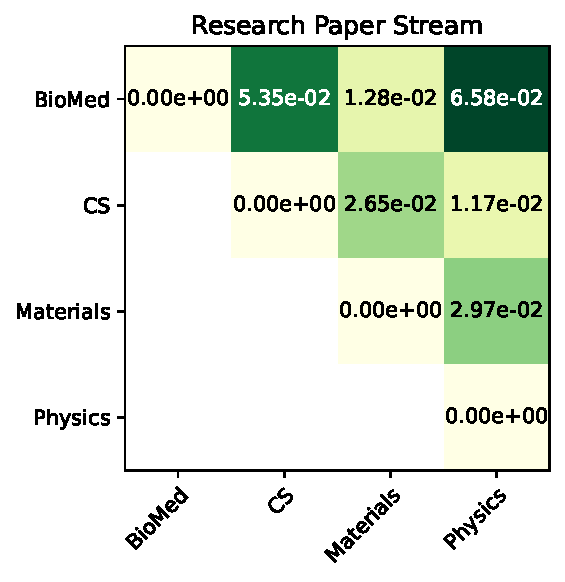
\includegraphics[width=0.80\linewidth]{acl2022/figs/dataset_analysis/sim_paper.pdf}}
    
    \subfloat[\scriptsize{Tweet Stream}]{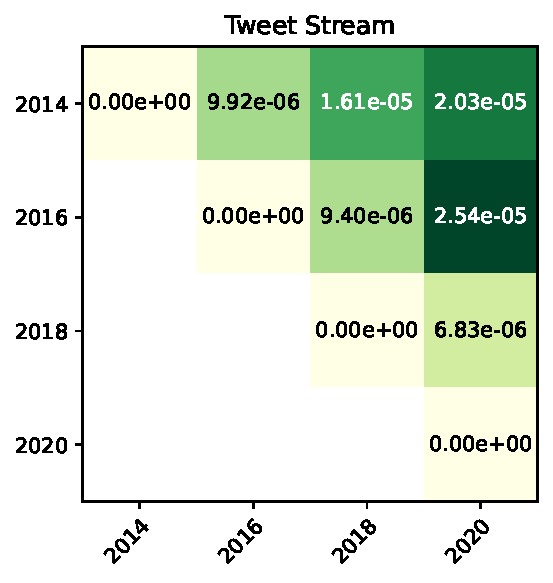
\includegraphics[width=0.80\linewidth]{acl2022/figs/dataset_analysis/sim_tweet.pdf}}

    % }
    \caption{Cosine distance of vocabulary distributions between each pair of datasets in two data streams.}
    \label{fig:vocab_sim_analysis}
\end{figure}

\section{Ethic Risks}
We would like to note that, in practice, continually pretrained models over real-world data streams would require identification and removal of biased contents from pretraining corpora, which may affect the prediction of downstream models. As PTLMs are continuously updated, the bias in earlier pretraining may have a profound negative impact. In future works, it is preferable to develop algorithms to ``forget'' certain biased knowledge from language models. We further note that any data released in this paper, especially the tweet stream, should only be used for research purposes.